

    \documentclass[11pt]{article}
    \usepackage{graphicx}
    \begin{document}
    \begin{titlepage}
    \title{\Huge ECS 171 Final Report}
    \author{\huge Aaun Abbas\\\huge Hilal Alsibai\\\huge Christopher Chen\\\huge Miguel Covarrubias\\\huge Jesse Dyer\\\huge Pei Guo\\\huge Alex Kot\\\huge Raymond Lau\\\huge Kent Wang\\\huge Ian Woods}
    \maketitle
    \end{titlepage}
    \section{Abstract}
    \paragraph{}
    In this project, we compared the effectiveness of several machine learning classifiers at determining forest cover types from cartographic variables. The classifiers we used were artificial neural networks, k nearest neighbors, and random forests. Our results showed that random forests more accurately predicted the correct forest cover type than any other classifier.
    \section{Introduction}
    \paragraph{}
    Determining forest cover type from purely cartographic variables is important in situations where it is unfeasible or impossible to obtain cover type data through empirical methods. Thus, being able to accurately estimate the cover type of an area is of great interest to forest scientists \cite{blackard00}. At the same time, the dataset provides a large amount of well structured data (581012 samples with 54 attributes) upon which different machine learning techniques can be tested and compared, making it an attractive dataset for computer scientists \cite{gama03,oza01,giannella,furnkranz,obradovic,klami}.
    \section{Methods}
    \paragraph{}
    We use three different classifiers to determine forest cover type: artificial neural networks, k nearest neighbors, and random forests.
    \subsection{Artificial Neural Networks}
    \subsection{k Nearest Neighbors}
    \paragraph{}
    The $k$-Nearest Neighbors (KNN) Algorithm involves classifying a given sample as a particular type, given the type of the $k$ closest samples to it, as determined by some distance function \cite{matlabpage}. Our initial approach was to use a standard Euclidean distance function, defined as follows \cite{sayad} :
    \\
    $\sqrt{\sum\limits_{k = 1}^n (x_{jk} - x_{ik})^2}$
    \\
    We decided to begin with this naive approach to isolate failure points (essentially, if something were to work incorrectly, we could rule out the distance function as failure point).
    We debated creating a distance function tailored to the dataset by hand, or by simply trying many different possible distance functions. However, we decided to generate a distance function with the largest-margin nearest neighbors algorithm (more precisely, we generated a transformation matrix that was used to transform the data, and still used the Euclidean distance).
    \\
    Using different values for $k$ can theoretically alter the predicted results - for example, if a sample of unknown type is closest to a sample of type $A$ with a calculated distance of 1, but two samples of type $B$ are at a distance of 1.1 from our unknown sample, choosing $k$ = 1 will yield the result $A$ for the unknown's type, and $k$ = 3 will yield the result $B$. We decided to test a wide range of $k$ values.
     
    \subsubsection{Brief Description of LMNN}
    \paragraph{}
    LMNN (Largest Margin Nearest Neighbors) is a variant of KNN that can be implemented in two ways. One method is to learn a Mahalanobis distance function, which measures the distance (in standard deviations) from the center of a cluster of similarly typed samples. Another method, and the method our implementation used, is to learn a transformation matrix that, when applied to the dataset, yields higher correct classification rates \cite{huyen12}. It learns this matrix by iteratively applying small perturbations to the transformation matrix with the goal of maintaining a large distance between "impostors" (close neighbors that are of the wrong type) and the perimeters that surround groups of similarly-typed neighbors. LMNN is very helpful because it saves use the trouble of testing many different distance functions \cite{weinberger}, or trying to derive a distance function by hand for each particular dataset. Pictured below are the results of our LMNN classifier, compared to the standard KNN classifier.
     
     
    \subsection{Random Forests}
    \paragraph{}
    We used Liaw and Wiener's R port \cite{liaw02} of Breiman's random forest algorithm \cite{breiman01}. Before training the classifier on the samples, we preprocessed the data so that the 4 boolean categorical variables that were related to wilderness area were rolled up into a single variable. We did the same for the 40 variables (also boolean categorical) that were related to soil type. This was done in order to speed up the training of the classifier.
    \par
    The random forest algorithm takes several parameters which control its speed and performance. We used empirical analysis to determine optimal values for these parameters. The first of these was $mtry$, which controls the number of variables that are sampled at each split when building the decision trees. 7 was determined to be the optimal value, as increasing the value past 7 caused almost no change in error, but consumed far more system resources. The other parameter was $ntree$ which controls the number of trees to be generated in the forest. For the same reasons as $mtry$, 40 was found to be the optimal value.
    \par
    To determine error, we used the OOB (out of bag) error \cite{breiman96}. We used this estimate because it is automatically generated by the algorithm while it runs, and because cross validation is not required when using OOB error, due to the way it is computed \cite{breiman01, breiman96}, which saved us computation time. It has also been shown to be close to an optimal estimate of the generalization error\cite{breiman96}.
    \section{Results}
    \subsection{KNN And LMNN Results}
    \subsubsection{Results of KNN Using Various K Values}
    \paragraph{}
    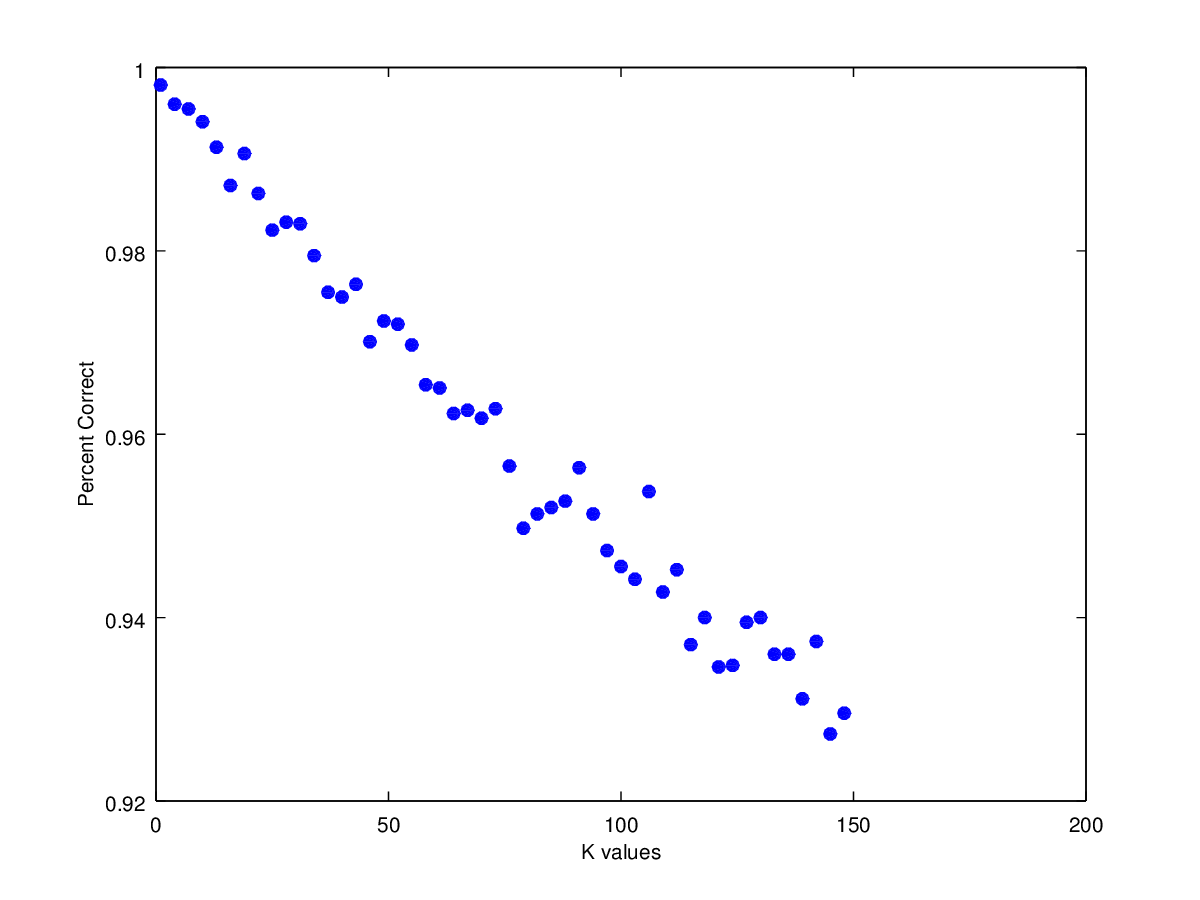
\includegraphics[scale=.66]{kValuesGraph.png}
    \\
    As can be seen in the above graph, increasing the value of $k$ reduced the accuracy of the classifier. We tested over a range from 1 to 150 with a step size of 3 (to reduce computation time while still revealing the overall trend). This makes intuitive sense - imagine a KNN implementation with $k = $ the size of the data set. Say there are $n$ samples of the most common type, and $z$ total samples. Every sample would be labeled as the most common sample, resulting in an accuracy of $\frac{n}{z}$.
    \subsubsection*{Results of LMNN}
    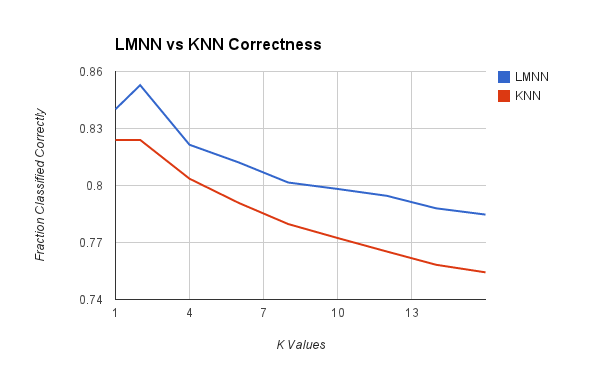
\includegraphics[scale=.66]{knnvslmnn.png}
    \paragraph{}
    LMNN was able to boost the correct classification percentage in every case. On average, we saw 2.46\% better classification rates. It took quite a lot of extra time to learn the distance function, though - running the LMNN algorithm on the entire UCI dataset took on the order of one hour on a relatively high-powered desktop computer (quad core Intel i5 processor at 3.4GHz, all CPUs at 95\% + load for most of the computation).
     
     
     
     
    \begin{figure}[htbp]
    \begin{minipage}[b]{\linewidth}
    \centering
    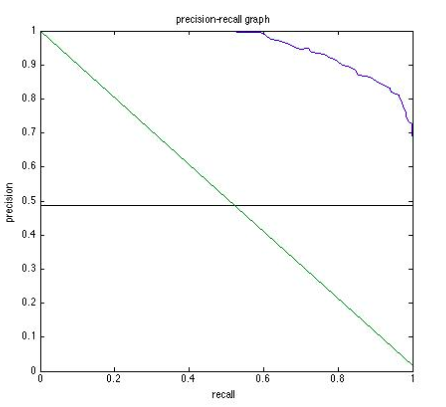
\includegraphics[width=\linewidth]{AspenPRCurve.png}
    \caption{PR Curve for class Aspen}
    \label{fig:chapter001_dist_001}
    \end{minipage}
    \end{figure}
    \hspace{0.5cm}
    \begin{figure}[htbp]
    \begin{minipage}[b]{\linewidth}
    \centering
    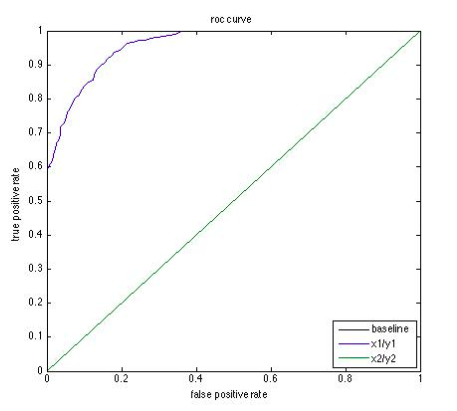
\includegraphics[width=\linewidth]{AspenROCCurve.png}
    \caption{ROC Curve for class Aspen}
    \label{fig:chapter001_reward_001}
    \end{minipage}
    \end{figure}
     
    \begin{figure}[htbp]
    \begin{minipage}[b]{\linewidth}
    \centering
    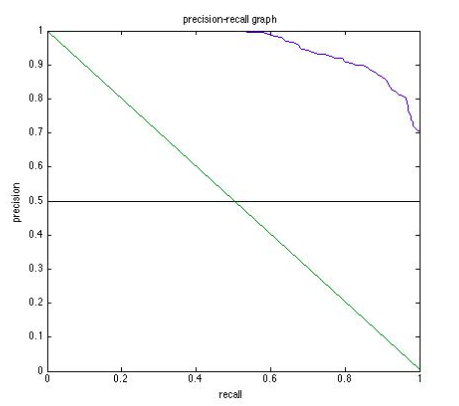
\includegraphics[width=\linewidth]{CottonwoodPRCurve.png}
    \caption{PR Curve for class Cottonwood}
    \label{fig:chapter001_dist_001}
    \end{minipage}
    \hspace{0.5cm}
    \end{figure}
    
    \begin{figure}[htbp]
    \begin{minipage}[b]{\linewidth}
    \centering
    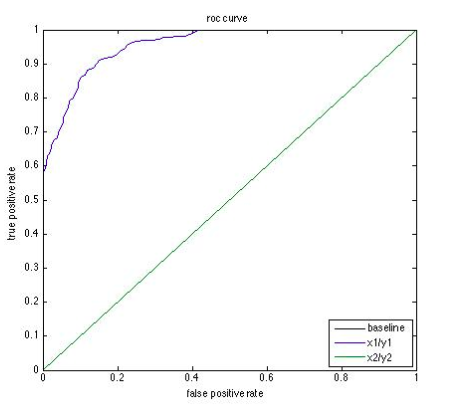
\includegraphics[width=\linewidth]{CottonwoodROCCurve.png}
    \caption{ROC Curve for class Cottonwood}
    \label{fig:chapter001_reward_001}
    \end{minipage}
    \end{figure}
     
    \begin{figure}[htbp]
    \begin{minipage}[b]{\linewidth}
    \centering
    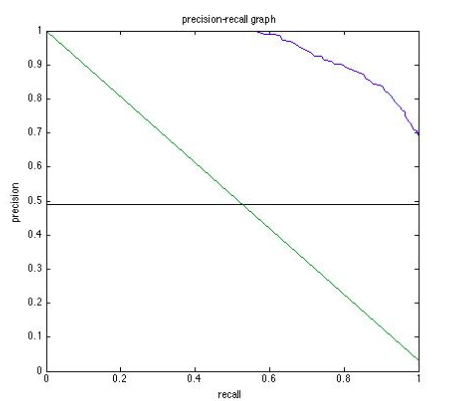
\includegraphics[width=\linewidth]{DouglasFirPRCurve.png}
    \caption{PR Curve for class Douglas Fir}
    \label{fig:chapter001_dist_001}
    \end{minipage}
    \hspace{0.5cm}
    \end{figure}
    \begin{figure}[htbp]
    \begin{minipage}[b]{\linewidth}
    \centering
    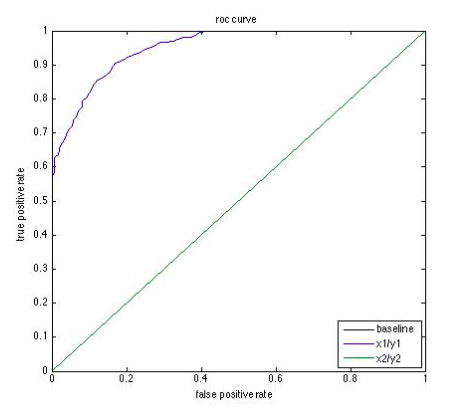
\includegraphics[width=\linewidth]{DouglasFirROCCurve.png}
    \caption{ROC Curve for class Douglas Fir}
    \label{fig:chapter001_reward_001}
    \end{minipage}
    \end{figure}
     
    \begin{figure}[htbp]
    \begin{minipage}[b]{\linewidth}
    \centering
    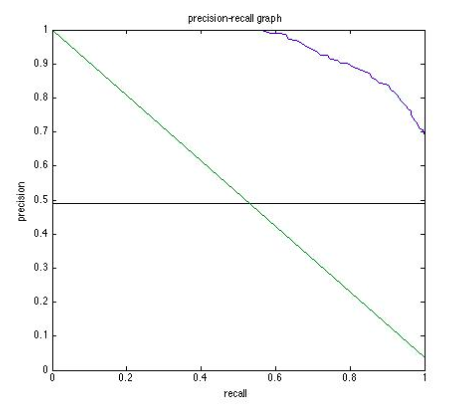
\includegraphics[width=\linewidth]{KrummholzPRCurve.png}
    \caption{PR Curve for class Krummholz}
    \label{fig:chapter001_dist_001}
    \end{minipage}
    \hspace{0.5cm}
    \end{figure}
    \begin{figure}[htbp]
    \begin{minipage}[b]{\linewidth}
    \centering
    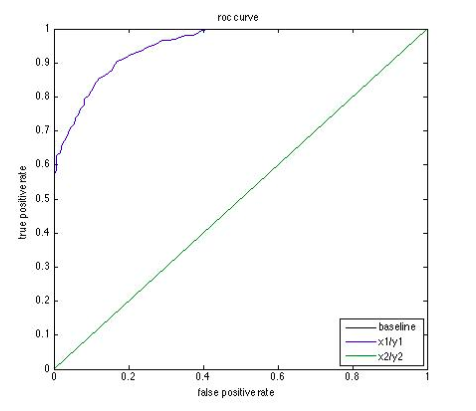
\includegraphics[width=\linewidth]{KrummholzROCCurve.png}
    \caption{ROC Curve for class Krummholz}
    \label{fig:chapter001_reward_001}
    \end{minipage}
    \end{figure}
     
    \begin{figure}[htbp]
    \begin{minipage}[b]{\linewidth}
    \centering
    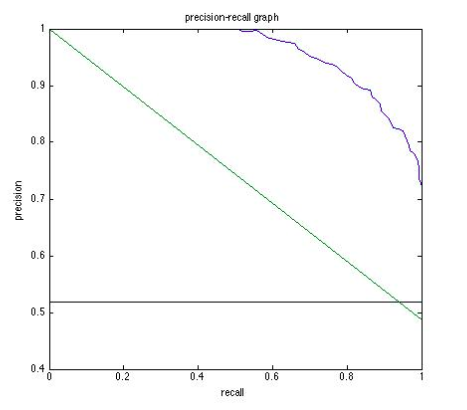
\includegraphics[width=\linewidth]{LodgepolePinePRCurve.png}
    \caption{PR Curve for class Lodgepole Pine}
    \label{fig:chapter001_dist_001}
    \end{minipage}
	\end{figure} 
    \hspace{0.5cm}
    \begin{figure}[htbp]
    \begin{minipage}[b]{\linewidth}
    \centering
    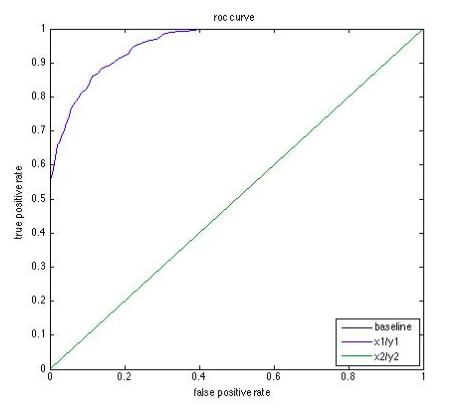
\includegraphics[width=\linewidth]{LodgepolePineROCCurve.png}
    \caption{ROC Curve for class Lodgepole Pine}
    \label{fig:chapter001_reward_001}
    \end{minipage}
    \end{figure}
     
    \begin{figure}[htbp]
    \begin{minipage}[b]{\linewidth}
    \centering
    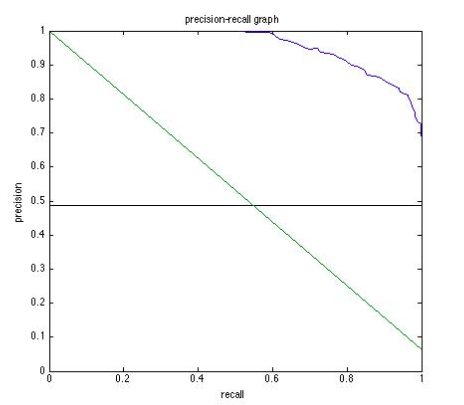
\includegraphics[width=\linewidth]{PonderosaPinePRCurve.png}
    \caption{PR Curve for class Ponderosa Pine}
    \label{fig:chapter001_dist_001}
    \end{minipage}
    \hspace{0.5cm}
    \end{figure}
    \begin{figure}[htbp]
    \begin{minipage}[b]{\linewidth}
    \centering
    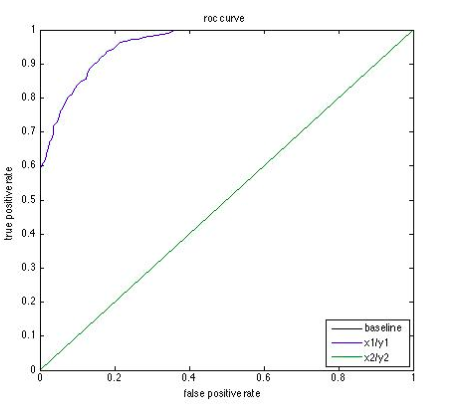
\includegraphics[width=\linewidth]{PonderosaPineROCCurve.png}
    \caption{ROC Curve for class Ponderosa Pine}
    \label{fig:chapter001_reward_001}
    \end{minipage}
    \end{figure}
     
    \begin{figure}[htbp]
    \begin{minipage}[b]{\linewidth}
    \centering
    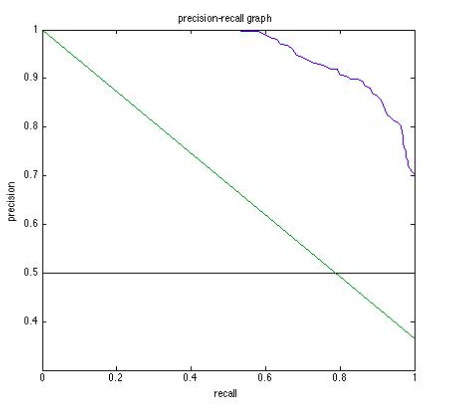
\includegraphics[width=\linewidth]{SpruceFirPRCurve.png}
    \caption{PR Curve for class Spruce Fir}
    \label{fig:chapter001_dist_001}
    \end{minipage}
    \hspace{0.5cm}
    \end{figure}
    \begin{figure}[htbp]
    \begin{minipage}[b]{\linewidth}
    \centering
    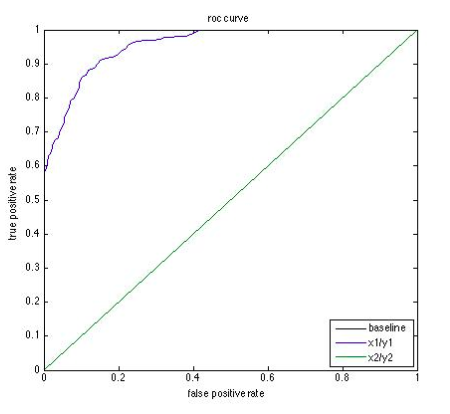
\includegraphics[width=\linewidth]{SpruceFirROCCurve.png}
    \caption{ROC Curve for class Spruce Fir}
    \label{fig:chapter001_reward_001}
    \end{minipage}
    \end{figure}
    \subsubsection{Final KNN and LMNN Analysis}
     
    \begin{center}
     \begin{tabular}{ l | r}
       \hline
       Cover Type & AUC \\ \hline
     
       Aspen & .892 \\ \hline
       Cottonwood & .877 \\ \hline
       Douglas Fir & .885 \\ \hline
       Krummholz & .888 \\ \hline
       Lodgepole Pine & .891 \\ \hline
       Ponderosa Pine & .883 \\ \hline
       Spruce Fir & .873 \\ \hline
     \end{tabular}
    \end{center}
    \paragraph{}
    From these graphs it can be seen that the performance from each of these classifiers is far greater than a random guess, and that they were also relatively consistent across the cover types.
     
    \section{Discussion}
    Why is one classifier better than another?
    \section{Conclusion}
    In this project we used 3 different classifiers to predict forest cover type based on cartographic variables: artificial neural networks, k nearest neighbors, and random forests. We determined that random forests outperformed the other 2 classifiers. In the future, we may try to examine the performance of these classifiers on other datasets and then compare those results to those given here, or we may use different classifiers on the cover type dataset to see if we can improve our classification accuracy.
    \section{Contributions}
    Aaun Abbas and Raymond Lau wrote all of the code that was related to random forests. Christopher Chen wrote all parts of the report that were related to random forests. Jesse Dyer wrote / gathered most of the code for the LMNN and KNN implementations. Ian Woods generated figures, ran computations, and wrote the report. Miguel Covarrubias ran computations and generated all ROC and PR curves.
    \pagebreak
    \begin{thebibliography}{}
    \bibitem{blackard00}
    Blackard, Jock A. and Denis J. Dean. 2000. "Comparative Accuracies of Artificial Neural Networks and Discriminant Analysis in Predicting Forest Cover Types from Cartographic Variables." Computers and Electronics in Agriculture 24(3):131-151.
    \bibitem{gama03}
    Joao Gama and Ricardo Rocha and Pedro Medas. Accurate decision trees for mining high-speed data streams. KDD. 2003.
    \bibitem{oza01}
    Nikunj C. Oza and Stuart J. Russell. Experimental comparisons of online and batch versions of bagging and boosting. KDD. 2001.
    \bibitem{giannella}
    Chris Giannella and Bassem Sayrafi. An Information Theoretic Histogram for Single Dimensional Selectivity Estimation. Department of Computer Science, Indiana University Bloomington.
    \bibitem{furnkranz}
    Johannes Furnkranz. Round Robin Rule Learning. Austrian Research Institute for Artificial Intelligence.
    \bibitem{obradovic}
    Zoran Obradovic and Slobodan Vucetic. Challenges in Scientific Data Mining: Heterogeneous, Biased, and Large Samples. Center for Information Science and Technology Temple University.
    \bibitem{klami}
    Arto Klami and Samuel Kaski and Ty n ohjaaja and Janne Sinkkonen. HELSINKI UNIVERSITY OF TECHNOLOGY Department of Engineering Physics and Mathematics Arto Klami Regularized Discriminative Clustering. Regularized Discriminative Clustering.
    \bibitem{liaw02}
    A. Liaw and M. Wiener (2002). Classification and Regression by randomForest. R News 2(3), 18--22.
    \bibitem{breiman01}
    Leo Breiman. Random forests. Machine learning 45 (1), 5-32. 2001.
    \bibitem{breiman96}
    Breiman, Leo. Out-of-bag estimation. Technical report, Statistics Department, University of California Berkeley, Berkeley CA 94708, 1996b. 33, 34, 1996.
    \bibitem{huyen12}
    Do, Huyen, et al. A metric learning perspective of SVM: on the relation of LMNN and SVM.
    \bibitem{matlabpage}
    http://www.mathworks.com/help/stats/knnsearch.html
    \bibitem{sayad}
    Dr Saed Sayad. K Nearest Neighbors, 2010, http://chem-eng.utoronto.ca/~datamining/Presentations/KNN.pdf
    \bibitem{weinberger}
    Weinberger, Kilian Q and Saul, Lawrence K. Distance Metric Learning for Large Margin
Nearest Neighbor Classification.
    \end{thebibliography}
    \end{document}

